\documentclass{beamer}
\usetheme{Madrid}
\usepackage{graphicx}
\usepackage{listings}
\usepackage{color}
\usepackage{caption}

\definecolor{codegreen}{rgb}{0,0.6,0}
\definecolor{codegray}{rgb}{0.5,0.5,0.5}
\definecolor{codepurple}{rgb}{0.58,0,0.82}
\definecolor{backcolour}{rgb}{0.95,0.95,0.92}

\lstdefinestyle{mystyle}{
    backgroundcolor=\color{backcolour},   
    commentstyle=\color{codegreen},
    keywordstyle=\color{magenta},
    numberstyle=\tiny\color{codegray},
    stringstyle=\color{codepurple},
    basicstyle=\ttfamily\footnotesize,
    breakatwhitespace=false,         
    breaklines=true,                 
    captionpos=b,                    
    keepspaces=true,                 
    numbers=left,                    
    numbersep=5pt,                  
    showspaces=false,                
    showstringspaces=false,
    showtabs=false,                  
    tabsize=2
}

\lstset{style=mystyle}

\title{Containers and Docker: An Introduction}
\date{\today}

\begin{document}

\frame{\titlepage}

\begin{frame}
\frametitle{What are Containers?}
\begin{itemize}
    \item A container is a lightweight, standalone package of software.
    \item It includes everything needed to run an app: code, runtime, system tools, libraries.
    \item Containers isolate applications from their environments.
    \item Think of them as a more efficient, minimal alternative to virtual machines.
\end{itemize}
\end{frame}

\begin{frame}
\frametitle{Why Use Containers?}
\begin{itemize}
    \item Portability — works on any system with a container runtime.
    \item Consistency — dev = test = prod.
    \item Speed — containers start in seconds.
    \item Efficiency — less overhead than full virtual machines.
\end{itemize}
\end{frame}

\begin{frame}
\frametitle{Containers vs Virtual Machines}
\centering
\begin{figure}
    \centering
    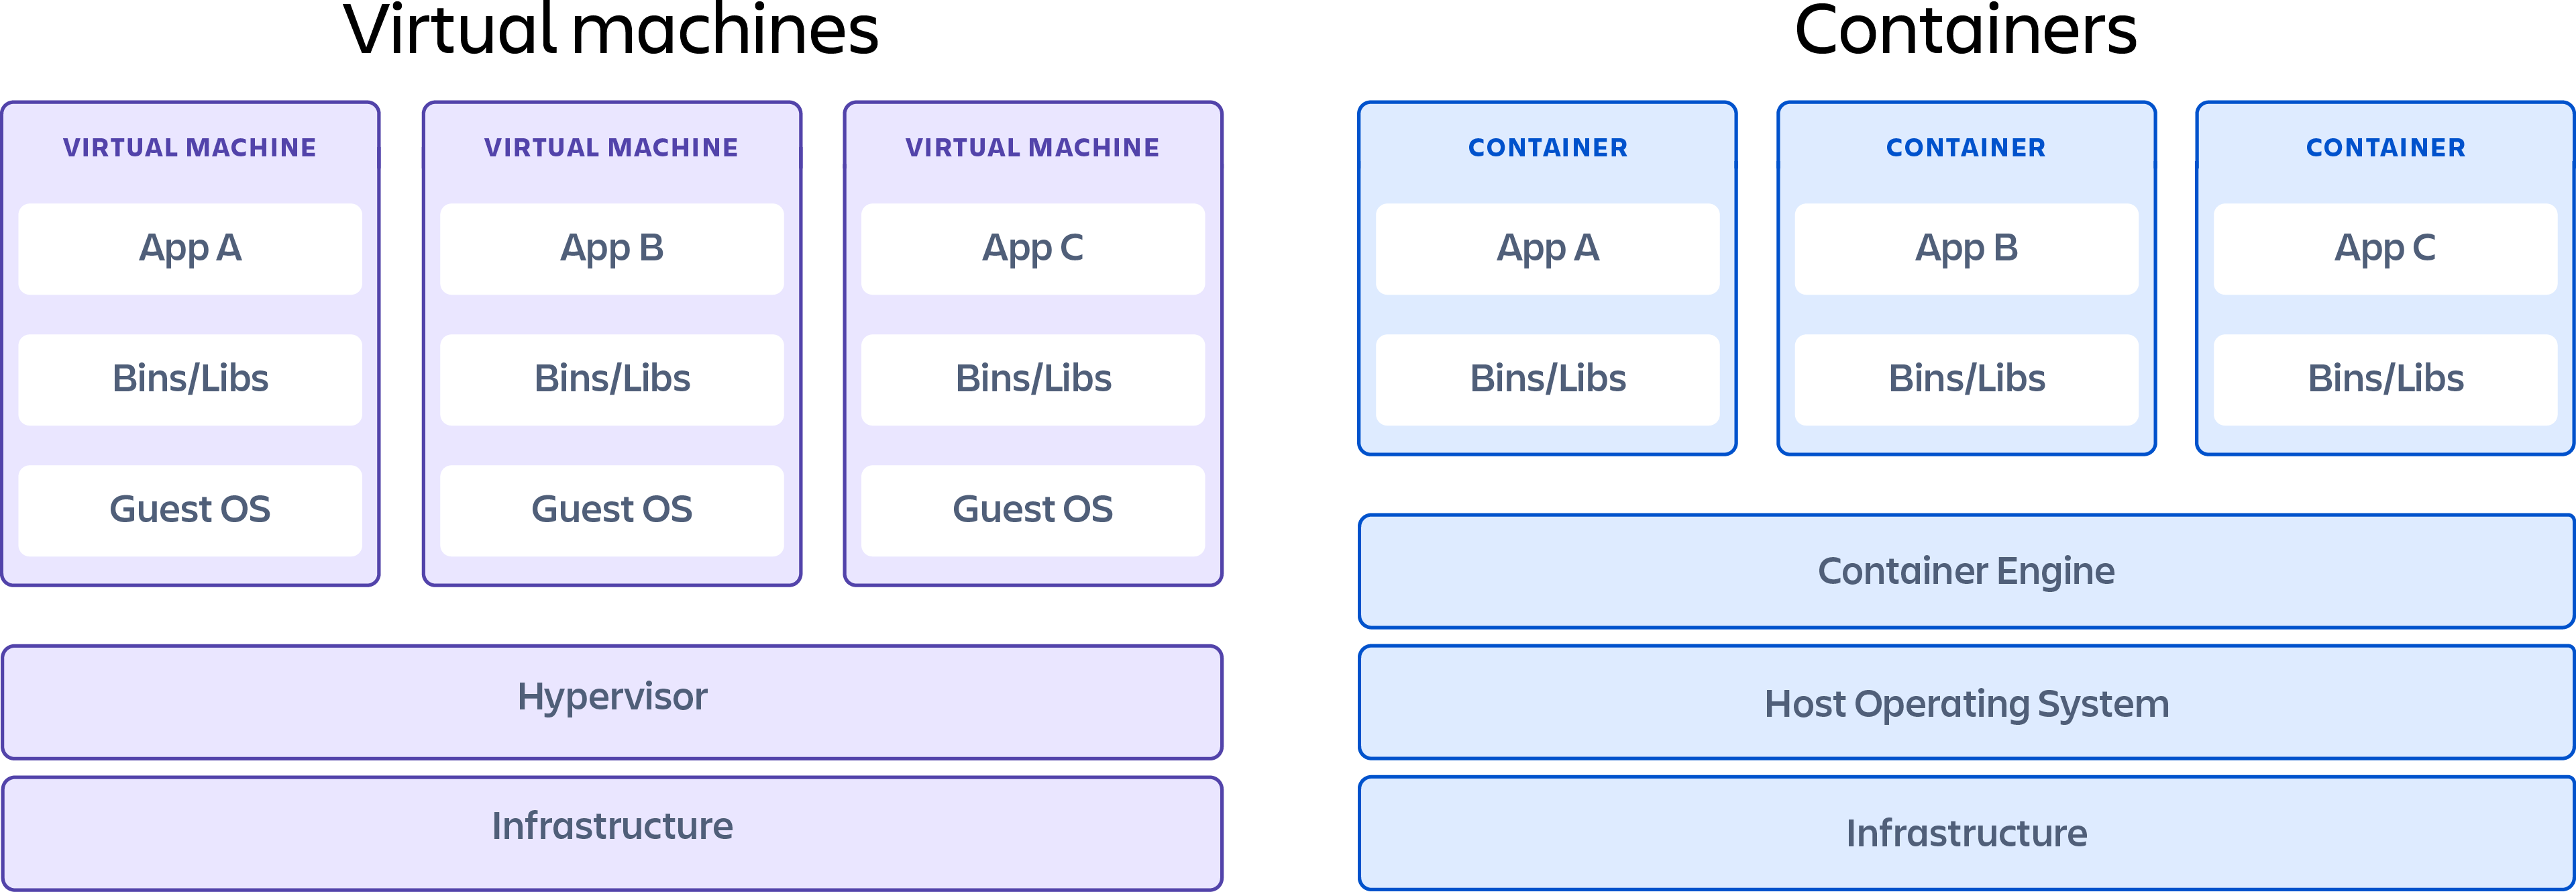
\includegraphics[width=0.9\linewidth]{images/image.png}
    \caption{VMs vs Containers — Key Architectural Differences}
    \label{fig:enter-label}
\end{figure}
\end{frame}

\begin{frame}
\frametitle{What is Docker?}
\begin{itemize}
    \item Docker is a platform that makes it easy to build, run, and manage containers.
    \item Provides CLI tools, image building, container lifecycle management, and orchestration support.
    \item Uses Dockerfiles to define container environments.
\end{itemize}
\end{frame}


\begin{frame}
\frametitle{Key Docker Terminology}
\begin{description}
  \item[Image] A read-only template used to create containers. It contains the app code, runtime, libraries, and dependencies.
  
  \item[Container] A runnable instance of an image. Containers are isolated, lightweight, and portable.

  \item[Dockerfile] A script of instructions to build a Docker image. Defines base image, files to copy, commands to run, etc.

  \item[Registry] A storage and distribution system for Docker images. Docker Hub is the default public registry.

  \item[Volume] A persistent storage mechanism for containers. Used to save data between container restarts.

  \item[Network] Docker allows isolated networks for containers to communicate securely.

  \item[Docker Engine] The runtime that builds and runs containers. It includes the daemon and CLI.

\end{description}
\end{frame}

\begin{frame}[fragile]
\frametitle{Basic Docker Commands}
\begin{lstlisting}[language=bash]
# Pull an image from the main registry
docker pull hello-world

# Run a container from an image
docker run hello-world

# List running containers
docker ps

# Stop and remove containers
docker stop container_id
docker rm container_id

\end{lstlisting}
\end{frame}

% Slide: Building Your Own Container
\begin{frame}[fragile]
\frametitle{Writing a Simple Dockerfile}
\begin{lstlisting}
# Use official Python image
FROM python:3.11-slim

# Set working directory
WORKDIR /app

# Copy local code
# the first . refers to the local files while the second is the destination inside the container
COPY . .

# Install dependencies
RUN pip install -r requirements.txt

# Run the app
CMD ["python", "main.py"]
\end{lstlisting}
\end{frame}

% Slide: Building and Running the Image
\begin{frame}[fragile]
\frametitle{Build and Run Your Image}
\begin{lstlisting}[language=bash]
# Build the Docker image
docker build -t my-python-app .

# Run it
docker run my-python-app
\end{lstlisting}
\end{frame}


\begin{frame}[fragile]
\frametitle{Advanced example}
\begin{lstlisting}[language=bash]
docker run -d --hostname my-rabbit \
           --name some-rabbit \
           -e RABBITMQ_DEFAULT_USER=user \
           -e RABBITMQ_DEFAULT_PASS=password \
           -p 5672:5672 \
           -p 15672:15672 \
           rabbitmq:3-management
\end{lstlisting}
\end{frame}

% Slide: Docker Compose
\begin{frame}
\frametitle{What is Docker Compose?}
\begin{itemize}
    \item Tool for defining and running multi-container applications.
    \item Configured using a `docker-compose.yml` file.
    \item Useful for setting up dev environments and microservices.
    \item Especially useful when running multiple containers that depend on each other.
    \item For more complicated configurations like the previous slide the commands can get tedious.
\end{itemize}
\end{frame}

% Slide: Docker Compose Example
\begin{frame}[fragile]
\frametitle{docker-compose.yml Example}
\begin{lstlisting}[language=yaml]
services:
  rabbitmq:
    image: rabbitmq:3-management
    container_name: some-rabbit
    hostname: my-rabbit
    environment:
      RABBITMQ_DEFAULT_USER: user
      RABBITMQ_DEFAULT_PASS: password
    ports:
      - "5672:5672"   # AMQP protocol
      - "15672:15672" # Management UI
    restart: unless-stopped
\end{lstlisting}

\begin{lstlisting}[language=bash]
# run the containers defined in the docker-compose.yml
docker compose up -d
\end{lstlisting}
\end{frame}


% Slide: Summary
\begin{frame}
\frametitle{Recap}
\begin{itemize}
    \item Containers isolate applications in lightweight environments.
    \item Docker simplifies working with containers.
    \item Dockerfiles define how to build images.
    \item Docker Compose manages multi-container setups.
\end{itemize}
\end{frame}

\begin{frame}
\frametitle{References}

\begin{itemize}
  \item Official Docker Documentation: \\
  \href{https://docs.docker.com}{\texttt{https://docs.docker.com}}

  \item Docker CLI Reference: \\
  \href{https://docs.docker.com/engine/reference/commandline/docker}{\texttt{docker command reference}}

  \item Docker Compose Docs: \\
  \href{https://docs.docker.com/compose/}{\texttt{https://docs.docker.com/compose/}}

  \item Dockerfile Reference: \\
  \href{https://docs.docker.com/engine/reference/builder/}{\texttt{https://docs.docker.com/engine/reference/builder/}}

  \item Atlassian: Containers vs. virtual machines: \\
  \href{https://www.atlassian.com/microservices/cloud-computing/containers-vs-vms}{ \scriptsize \texttt{https://www.atlassian.com/microservices/cloud-computing/containers-vs-vms}}
\end{itemize}

\end{frame}

% Slide: Questions
\begin{frame}
\frametitle{Q \& A}
\centering
{\Huge Questions?}
\end{frame}

\end{document}
